\documentclass[conference]{IEEEtran}

\usepackage{cite}
\usepackage{amsmath,amssymb,amsfonts}
\usepackage{graphicx}
\usepackage{textcomp}
\usepackage{xcolor}
\usepackage{url}
\usepackage[caption=false,font=footnotesize]{subfig}
\usepackage{multirow}

\graphicspath{{../../article/}}

\title{AI-based Pipeline for Handwritten Diagram Digitalization (DRAFT)}

\author{
    \IEEEauthorblockN{Saverio Napolitano}
    \IEEEauthorblockA{
        \textit{Dept. of Engineering Enzo Ferrari} \\
        \textit{Univ. of Modena and Reggio Emilia} \\
        Modena, Italy \\
        https://orcid.org/0009-0001-7847-456X
    }
    \and
    \IEEEauthorblockN{Nicola Ricciardi}
    \IEEEauthorblockA{
        \textit{Dept. of Engineering Enzo Ferrari} \\
        \textit{Univ. of Modena and Reggio Emilia} \\
        Modena, Italy \\
        https://orcid.org/0009-0006-3311-6669
    }
    \and
     \IEEEauthorblockN{Filippo Garagnani}
    \IEEEauthorblockA{
        \textit{Dept. of Engineering Enzo Ferrari} \\
        \textit{Univ. of Modena and Reggio Emilia} \\
        Modena, Italy \\
        https://orcid.org/0009-0003-3012-6042
    }
}

\begin{document}
\bstctlcite{IEEEexample:BSTcontrol}

\maketitle

\begin{abstract}
In engineering education, handwritten diagrams are widely used to express algorithms, workflows, state machines, and system structures. These artifacts support reasoning during exercises and project work, but they are difficult to edit, archive, reuse, or integrate into digital learning material when they exist only on paper or in static photographs. This paper presents DRAFT (Diagram Recognition and Formatting Tool), an AI-assisted system for converting handwritten engineering diagrams into structured and editable digital representations. The pipeline combines diagram classification, object detection, optical character recognition, and deterministic post-processing to generate markup-based outputs such as Mermaid and D2. The contribution is a modular tool for supporting documentation, revision, and future feedback workflows in engineering education, demonstrated through component-level metrics and qualitative end-to-end examples.
\end{abstract}


\begin{IEEEkeywords}
engineering education, handwritten diagram recognition, AI-assisted learning tools
\end{IEEEkeywords}

\section{Introduction}
Diagrams are central to engineering education. Students and instructors routinely use flowcharts, state diagrams, process sketches, and graph-like structures to reason about algorithms, systems, and behaviors. These representations are effective for rapid thinking and communication, but they often remain locked in notebooks, scans, or smartphone photographs. As a result, they are difficult to revise, include in digital reports, reuse in course material, or process in later feedback workflows.

Converting handwritten diagrams into editable digital formats can support multiple educational needs. Students can refine and document their work more easily, instructors can archive diagram-based submissions in structured form, and future tools can build on the extracted representation for semi-automatic feedback or assessment. However, this conversion requires several non-trivial steps, including diagram-type recognition, element detection, text digitization, and relation reconstruction.

This paper presents DRAFT (Diagram Recognition and Formatting Tool), an AI-assisted tool for converting handwritten engineering diagrams into structured and editable digital representations through a modular pipeline that combines learned and deterministic components to support diagram-based learning workflows.

More specifically, the paper contributes:
\begin{itemize}
\item a modular pipeline that converts handwritten engineering diagrams into editable Mermaid and D2 representations;
\item a combined evaluation that integrates classifier, detection, and OCR results with end-to-end qualitative examples;
\item a qualitative comparison with zero-shot GPT-4o that shows the task-specific pipeline better preserves node shapes and relational structure in the generated markup.
\end{itemize}

\section{Related Work}
Research on handwritten diagrams spans document analysis, sketch understanding, and structured diagram generation. Deep-learning approaches have been used to recognize arrow-oriented diagrams, as in Arrow R-CNN \cite{arrowrcnn}, and recent work has explored sketch-to-diagram conversion into vector formats \cite{sketchdiagram}. Earlier interactive systems also addressed hand-drawn UML recognition \cite{interactiveUML}. In parallel, online handwritten-diagram recognition has benefited from stroke order and pen trajectory information \cite{online1,online2,online3,framework}, whereas the present work addresses the more challenging offline setting in which only an image of the final handwritten diagram is available.

From an educational perspective, diagrams are not only visual recognition targets but also learning artifacts. Educational diagrams encode structure, process, and reasoning \cite{ai2d}, and tools for turning sketches into structured forms suggest clear value for engineering and software-related learning activities \cite{interactiveUML,modelsketch}. Recent engineering education research also reflects growing interest in AI-assisted tools for feedback, software engineering learning, and engineering drawing support \cite{isetGenAISE,inquisitiveAI,genAIDrawingsFeedback}. DRAFT is positioned within this space as a task-specific educational tool rather than a benchmark-driven computer vision contribution.

\section{System Architecture}
Figure~\ref{fig:pipeline} shows the overall architecture. The pipeline is composed of four main modules: Classifier, Extractor, Transducer, and Compiler.

\begin{figure}[htbp]
\centering

\includegraphics[width=\linewidth]{overview.png}
\caption{Overview of the DRAFT architecture.}
\label{fig:pipeline}
\end{figure}

The \textbf{Classifier} determines the category of the submitted handwritten diagram (flowchart, graph, or other) and routes it to the appropriate extraction pipeline. It operates on preprocessed images (grayscale, binarized, perspective-corrected) using a compact CNN, chosen lightweight because routing among three broad diagram categories is a simpler task than the downstream extraction. The \textbf{Extractor} applies Faster R-CNN object detection and TrOCR optical character recognition, then runs deterministic post-processing to build a unified, category-agnostic internal representation consisting of \textit{elements} (nodes with attached text) and \textit{relations} (arrows with source, target, and optional label); this shared format is what allows a single Transducer to generate markup for multiple diagram types. The \textbf{Transducer} converts this representation into Mermaid or D2 markup. The \textbf{Compiler} renders the final digital diagram. The output is an editable artifact that can be revised, documented, and reused in digital course material.

\section{System Implementation}
The current implementation focuses on handwritten flowcharts and graph-like diagrams. For classification, input images are preprocessed via grayscale conversion, Otsu binarization, median filtering (kernel 3, to remove checkered notebook patterns), perspective correction, and padding, as summarized in Fig.~\ref{fig:preprocessing}. The CNN consists of three convolutional blocks (8, 16, and 24 output channels, each followed by batch normalization and max pooling) and three fully connected layers (2048, 128, and 3 units, dropout 0.2). Initial experiments with a smaller two-layer architecture (AlexNet-style) and standard cross-entropy yielded a validation loss stagnating at 0.9 — above the random-guessing baseline of $-\ln 3 \approx 1.1$ but insufficient for reliable classification. Adding a third convolutional layer did not improve results; the root cause was class imbalance, with the \textit{other} category dominating the training set. The final model is trained for 10 epochs with AdamW (lr\,=\,0.001) using weighted cross-entropy; weights are set to the inverse of each class's normalized frequency.

\begin{figure}[htbp]
\centering
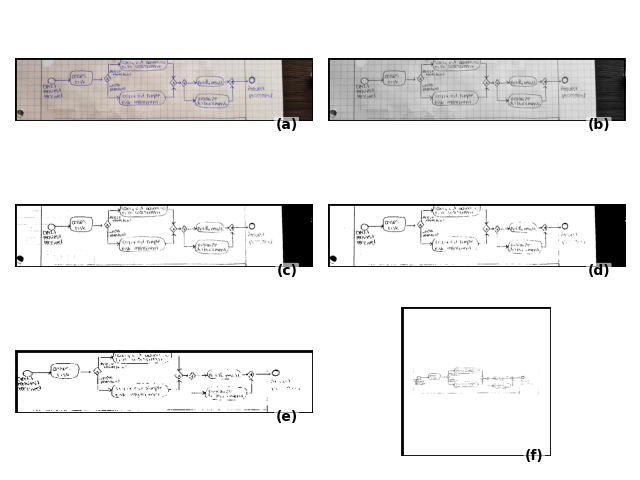
\includegraphics[width=\linewidth]{classifier_preprocessing.png}
\caption{Classifier preprocessing sequence used to normalize classroom-style input images.}
\label{fig:preprocessing}
\end{figure}

For extraction, DRAFT uses Faster R-CNN with a ResNet-50 FPN backbone \cite{rcnn,lin2017feature}, pretrained on COCO \cite{coco} and fine-tuned for 100 epochs (lr\,=\,0.005) on flowchart and graph diagram data. Unlike classifier preprocessing, extraction applies only a grayscale conversion: experiments showed that additional filters degrade OCR accuracy on handwritten text regions. The detector identifies nodes, arrows (body, head, tail), and text regions. OCR is performed with TrOCR base handwritten \cite{microsofttrocr}. Deterministic post-processing handles three tasks. First, \textit{arrow recovery}: when head or tail detections are missing for an arrow body, the detector is re-applied to an expanded crop around the body; the highest-confidence result above a confidence threshold is retained. For orphan head-tail pairs with no matching body, the region between them is cropped and re-queried; a candidate body is accepted only if its IoU with both bounding boxes exceeds a threshold. Second, \textit{relationship building}: source and target elements for each arrow are assigned by minimum distance from head and tail to node centers, with associations beyond a configurable distance threshold discarded. Third, \textit{text association}: text is linked to the nearest element. For nodes, bounding-box overlap between the text and node regions determines placement: overlap above a threshold classifies the text as inside; otherwise, the centroid distance must fall below a second threshold for the association to be retained as outside. For arrows, the distance between the text and the head-to-tail segment is first compared against a threshold; associations that exceed it are discarded. The segment is then split into three sections — the central section intentionally larger than the head and tail sections — and the text is assigned to the section of minimum distance. Self-arrows use a triangle approximation — two segments with the third vertex at the midpoint of the opposing bounding-box edge — since a single-segment line is inaccurate for arcs. The resulting internal representation is translated into Mermaid or D2 markup and rendered as a digital diagram. Fig.~\ref{fig:textassoc} illustrates the two geometric approximations used in text association.

{\setlength{\intextsep}{2pt}
\begin{figure}[!h]
    \centering
    \vspace{-1em}
    \subfloat[Arrow 3-split]{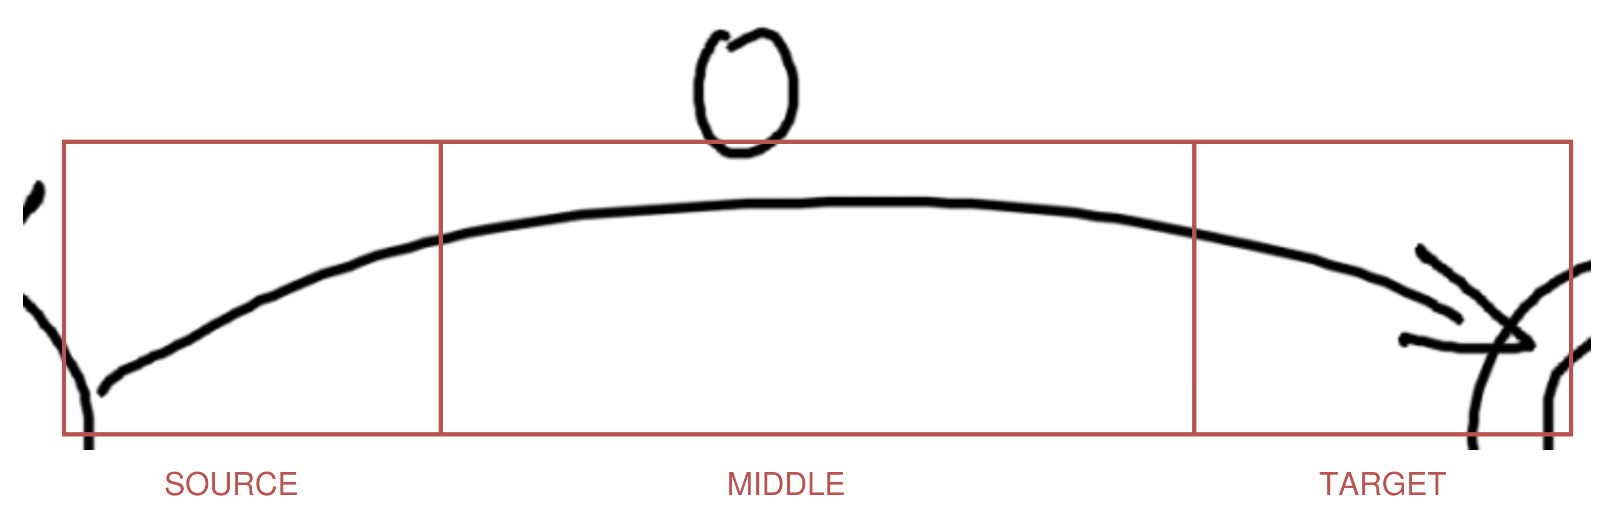
\includegraphics[width=0.45\linewidth,trim={0 0 0 30pt},clip]{arrowsplit.jpg}}
    \hfill
    \subfloat[Self-arrow triangle]{\includegraphics[width=0.45\linewidth]{self_arrow_crop.png}}
    \caption{Text association geometry: (a) arrow segment split into head, body, and tail sections; (b) self-arrow approximated as two segments for distance computation.}
    \label{fig:textassoc}
\end{figure}}

The internal representation is organized around elements and relations. Elements include diagram nodes and attached text, while relations encode arrows, source and target assignments (either of which may be absent for partial arrows), and optional labels. This representation is intentionally diagram-oriented rather than pixel-oriented, because the educational objective is to produce editable structures that can be revised by students or reused by instructors. Fig.~\ref{fig:extractor} summarizes the main flowchart extraction stages.

\begin{figure}[htbp]
\centering
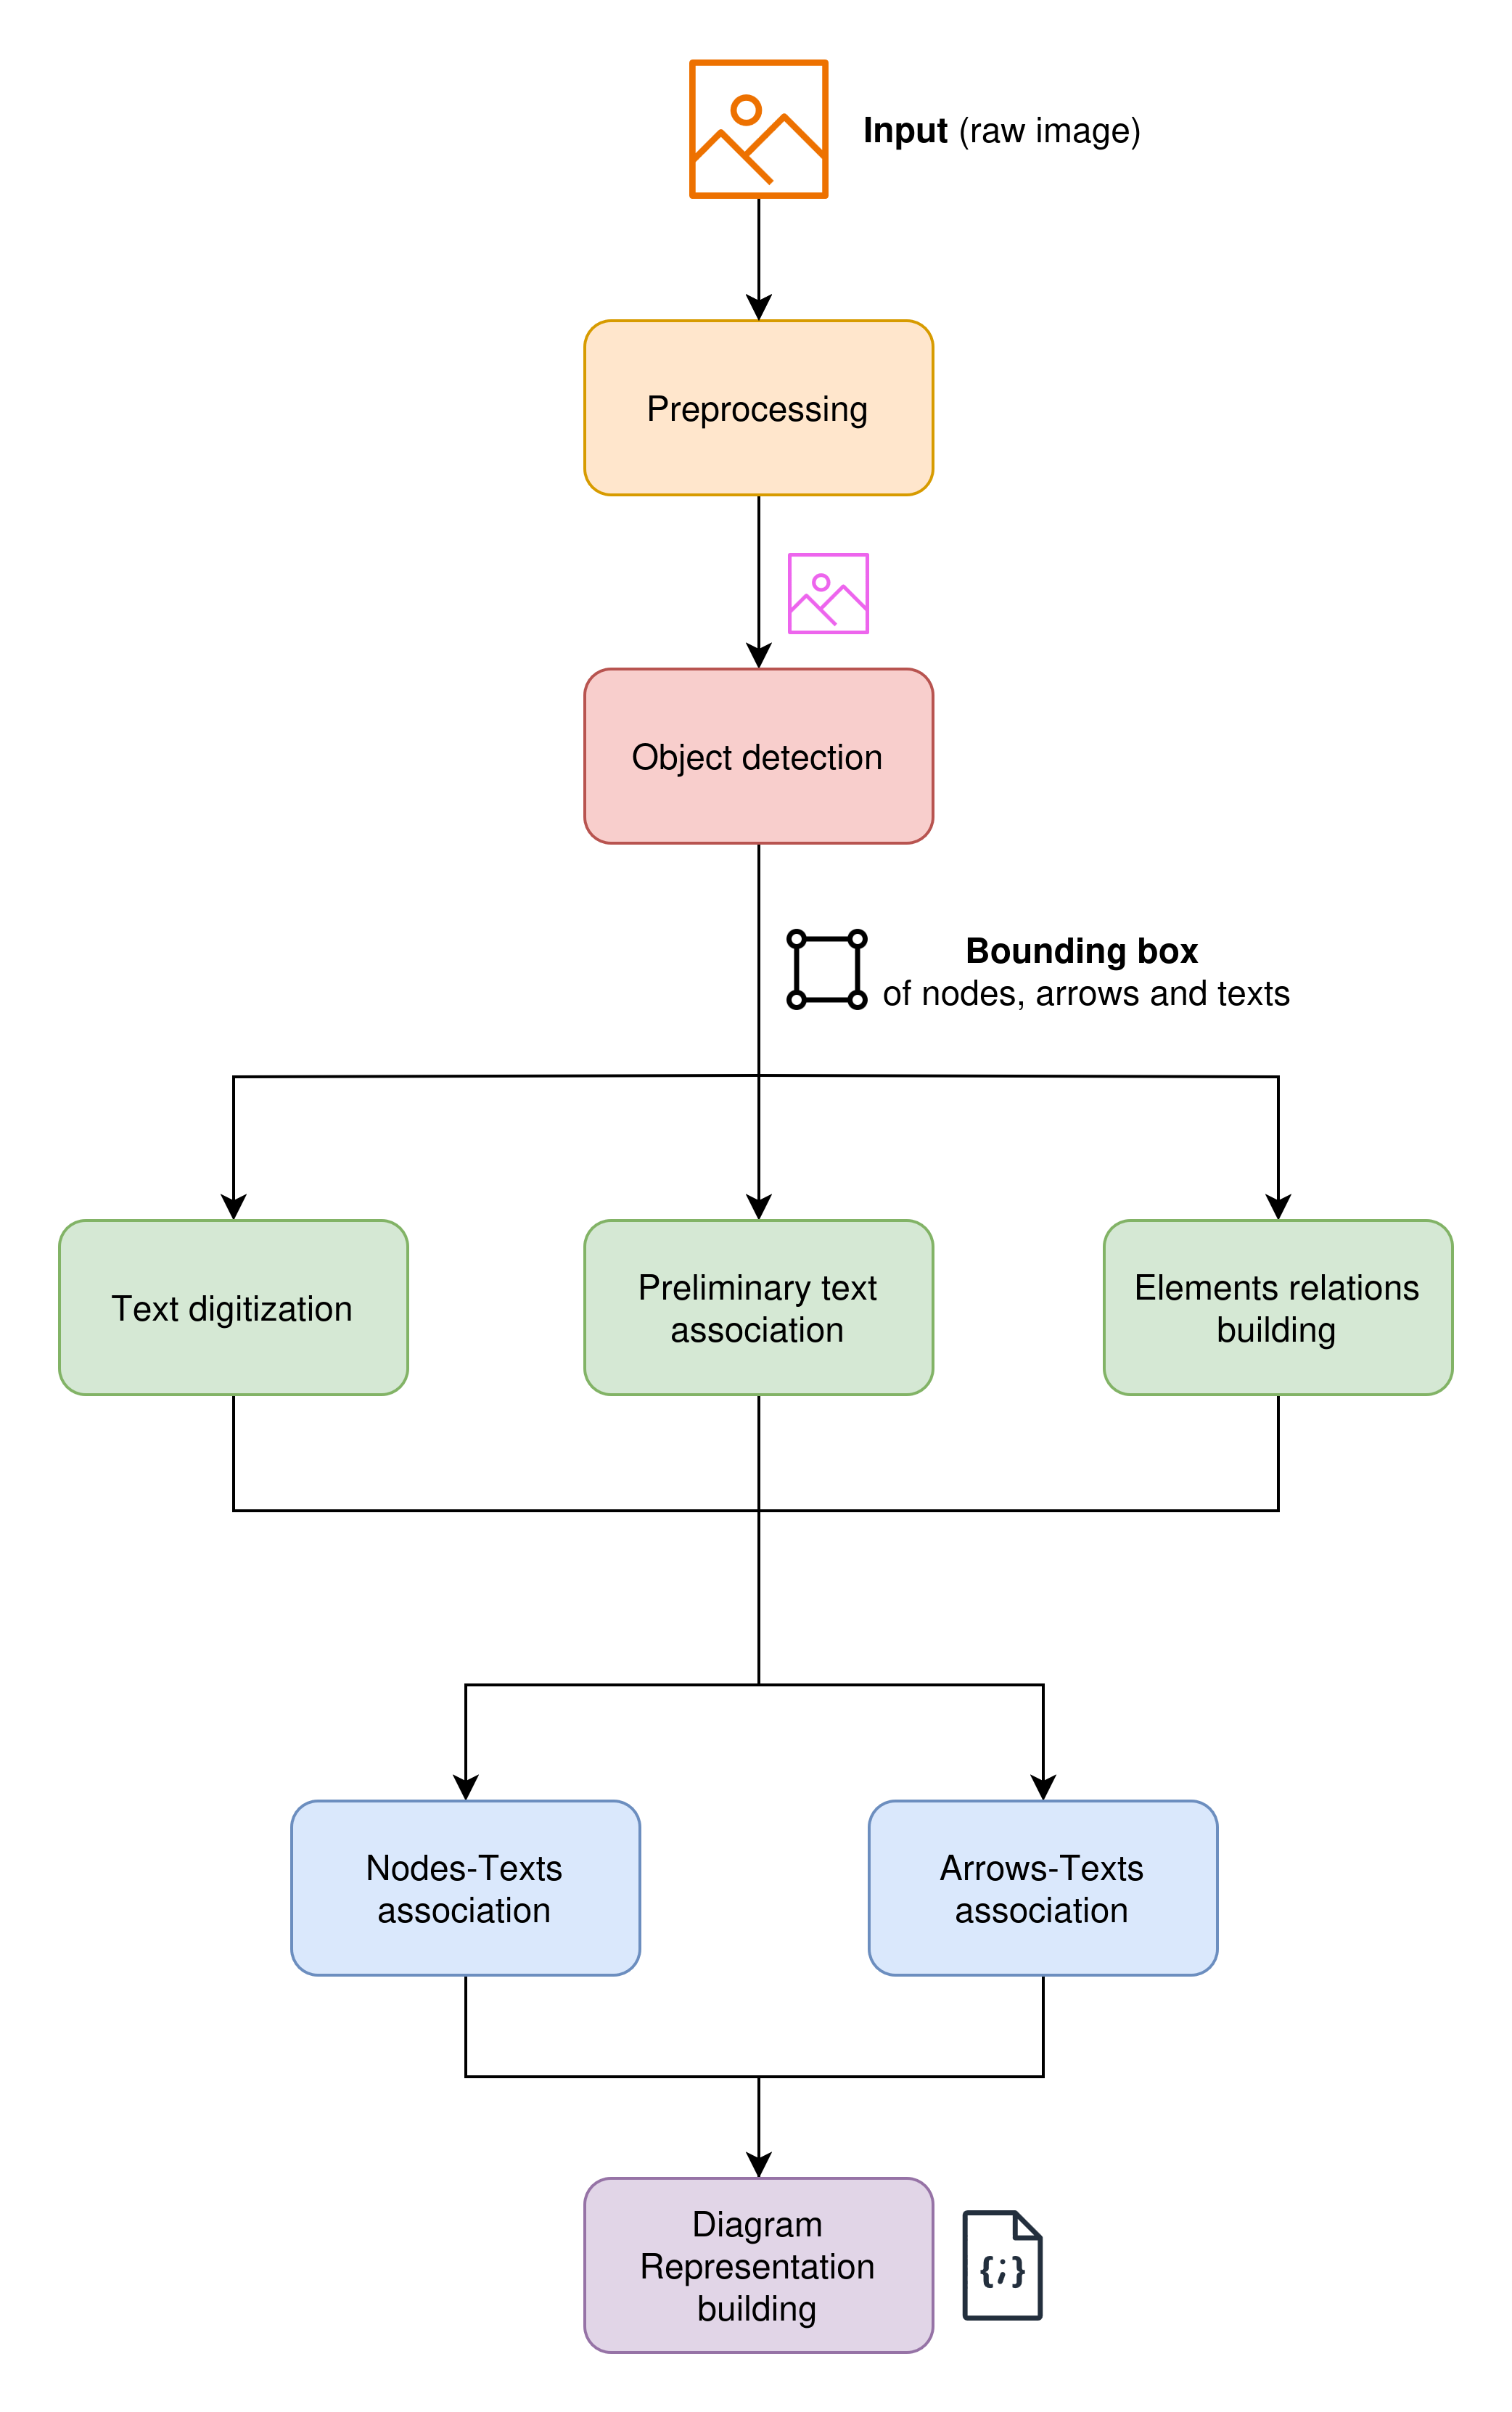
\includegraphics[width=\linewidth]{flowchart-extractor.png}
\caption{Main stages of the flowchart extraction process.}
\label{fig:extractor}
\end{figure}

To improve robustness across student-generated material, DRAFT draws on six public handwritten-diagram datasets (Table~\ref{tab:datasets}). Classifier training uses UML class diagrams, circuit diagrams, and educational science diagrams \cite{modelsketch,circuitnet,ai2d} as negative examples for the \textit{other} class, together with the same flowchart and graph data used for extraction. Extraction training focuses on the Finite Automata, FCB, and OHFCD\_1 datasets \cite{online1,online3,ohfcd}. This split reflects the intended use case: heterogeneous uploads require a broad classifier, while supported diagram types benefit from specialized extraction training.

\begin{table}[htbp]
\centering
\caption{Datasets used by DRAFT.}
\label{tab:datasets}
\begin{tabular}{|l|l|l|}
\hline
\textbf{Dataset} & \textbf{Use} & \textbf{Type} \\
\hline
Finite Automata \cite{online1} & Extraction & Graph/FA \\
FCB \cite{online3}             & Extraction & Flowchart \\
OHFCD\_1 \cite{ohfcd}          & Extraction & Flowchart \\
UML Class Diagrams \cite{modelsketch} & Classifier & Class diagrams \\
CircuitNet \cite{circuitnet}   & Classifier & Circuit diagrams \\
AI2D \cite{ai2d}               & Classifier & Science diagrams \\
\hline
\end{tabular}
\end{table}

\section{System Evaluation}
The evaluation combines component-level metrics with qualitative end-to-end examples to assess the suitability of the system as an educational tool.

\begin{table}[htbp]
\centering
\caption{Object detection mAP metrics (100-epoch fine-tuned model).}
\label{tab:map}
\begin{tabular}{|l|c|l|}
\hline
\textbf{Metric} & \textbf{Value} & \textbf{Scope} \\
\hline
mAP       & 0.8754 & Overall \\
mAP@0.5   & 0.9878 & IoU threshold 0.5 \\
mAP@0.75  & 0.9183 & IoU threshold 0.75 \\
\hline
mAP (Small)  & 0.6444 & Small objects \\
mAP (Medium) & 0.8054 & Medium objects \\
mAP (Large)  & 0.8975 & Large objects \\
\hline
\end{tabular}
\end{table}

\begin{table}[htbp]
\centering
\caption{Object detection mAR metrics (100-epoch fine-tuned model).}
\label{tab:mar}
\begin{tabular}{|l|c|l|}
\hline
\textbf{Metric} & \textbf{Value} & \textbf{Scope} \\
\hline
mAR@1   & 0.3436 & Max 1 detection/image \\
mAR@10  & 0.8877 & Max 10 detections/image \\
mAR@100 & 0.9128 & Max 100 detections/image \\
\hline
mAR (Small)  & 0.6631 & Small objects \\
mAR (Medium) & 0.8670 & Medium objects \\
mAR (Large)  & 0.9141 & Large objects \\
\hline
\end{tabular}
\end{table}

The classifier initially suffered from class imbalance because the \textit{other} category dominated the training set. Weighted cross-entropy substantially improved performance, yielding 97\% validation accuracy. For extraction, the detector was evaluated at three training stages — zero-shot (COCO weights only), 10-epoch, and 100-epoch fine-tuning — with the 100-epoch model selected based on detection completeness (Fig.~\ref{fig:detection}). The final model achieved the results shown in Tables~\ref{tab:map} and~\ref{tab:mar}. Performance degrades on small objects (mAP 0.6444), reflecting the difficulty of detecting fine-grained diagram elements at low resolution. Average localization errors were 6.84 px (x) and 4.84 px (y). The low mAR@1 (0.3436) is expected: the single-detection cap is trivially insufficient for diagrams with dozens of elements.

For OCR, several TrOCR variants were compared on handwritten diagram text. The \textit{base handwritten} model produced the best cosine and Euclidean distance scores, while the \textit{small handwritten} model yielded the best Hamming distance. In this work, this comparison was used as a practical model-selection step rather than as a standalone research contribution; Table~\ref{tab:ocr} reports the comparison, and Figs.~\ref{fig:ocr_examples} and~\ref{fig:ocr_failures} show representative easy and difficult cases.

\begin{table}[htbp]
\centering
\caption{OCR model comparison on handwritten diagram text.}
\label{tab:ocr}
\begin{tabular}{|l|c|c|c|}
\hline
\textbf{Model} & \textbf{Hamming} & \textbf{Cosine} & \textbf{Euclidean} \\
\hline
TrOCR small printed & 1.392 & 0.150 & 7133 \\
TrOCR small handwritten & \textbf{1.346} & 0.100 & 3947 \\
TrOCR base handwritten & 1.549 & \textbf{0.057} & \textbf{3003} \\
\hline
\end{tabular}
\end{table}

\begin{figure}[htbp]
\centering
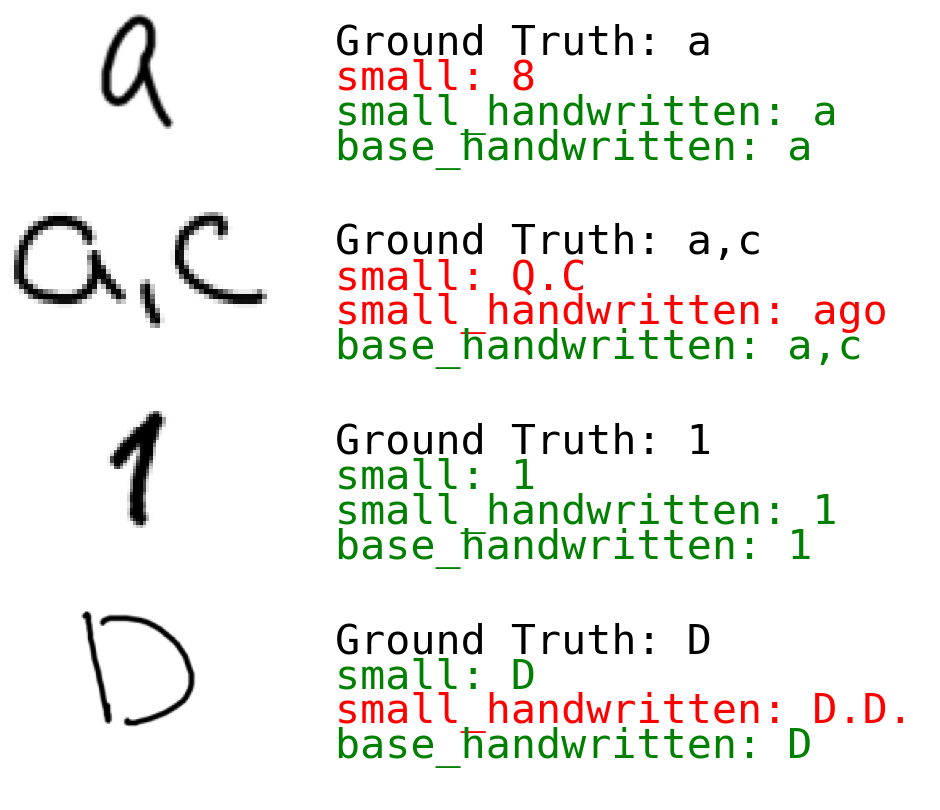
\includegraphics[width=\linewidth]{text_digitization_results_1.png}
\caption{Representative OCR outputs on handwritten diagram text regions.}
\label{fig:ocr_examples}
\end{figure}

\begin{figure}[htbp]
\centering
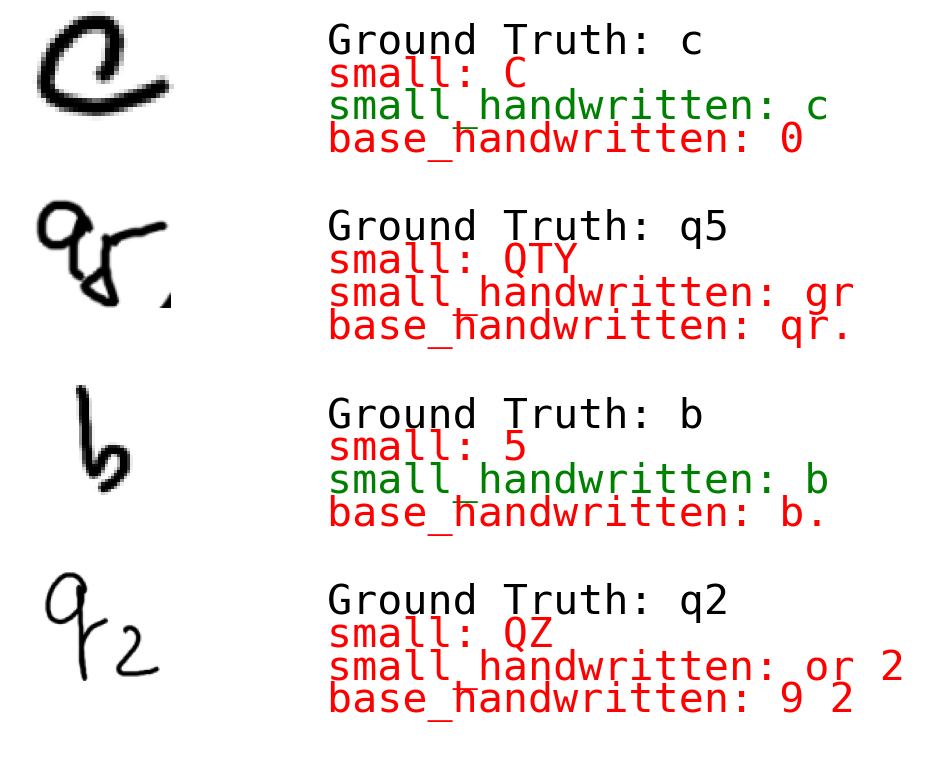
\includegraphics[width=\linewidth]{text_digitization_results_2.png}
\caption{Examples of more difficult handwritten text regions for OCR.}
\label{fig:ocr_failures}
\end{figure}

\begin{figure}[htbp]
    \centering
    \subfloat[Graph input]{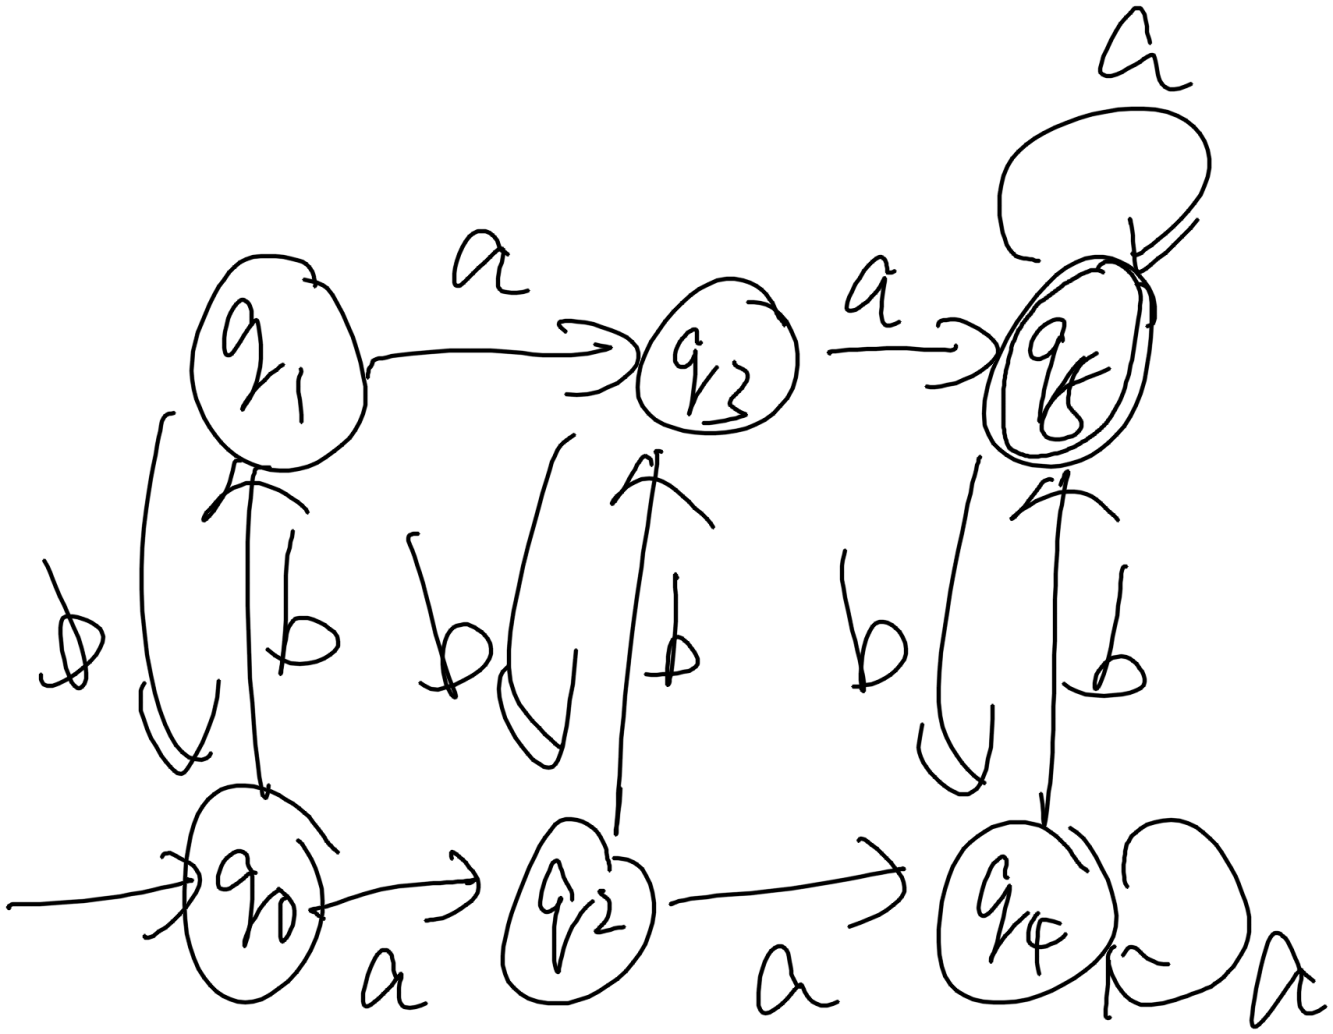
\includegraphics[width=0.44\linewidth]{ex3.png}}
    \hfill
    \subfloat[Structured output]{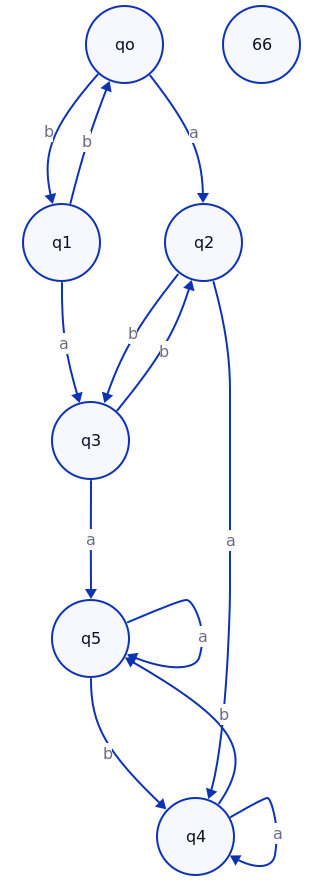
\includegraphics[width=0.18\linewidth]{ex4.png}}

    \vspace{0.6em}

    \subfloat[Flowchart input]{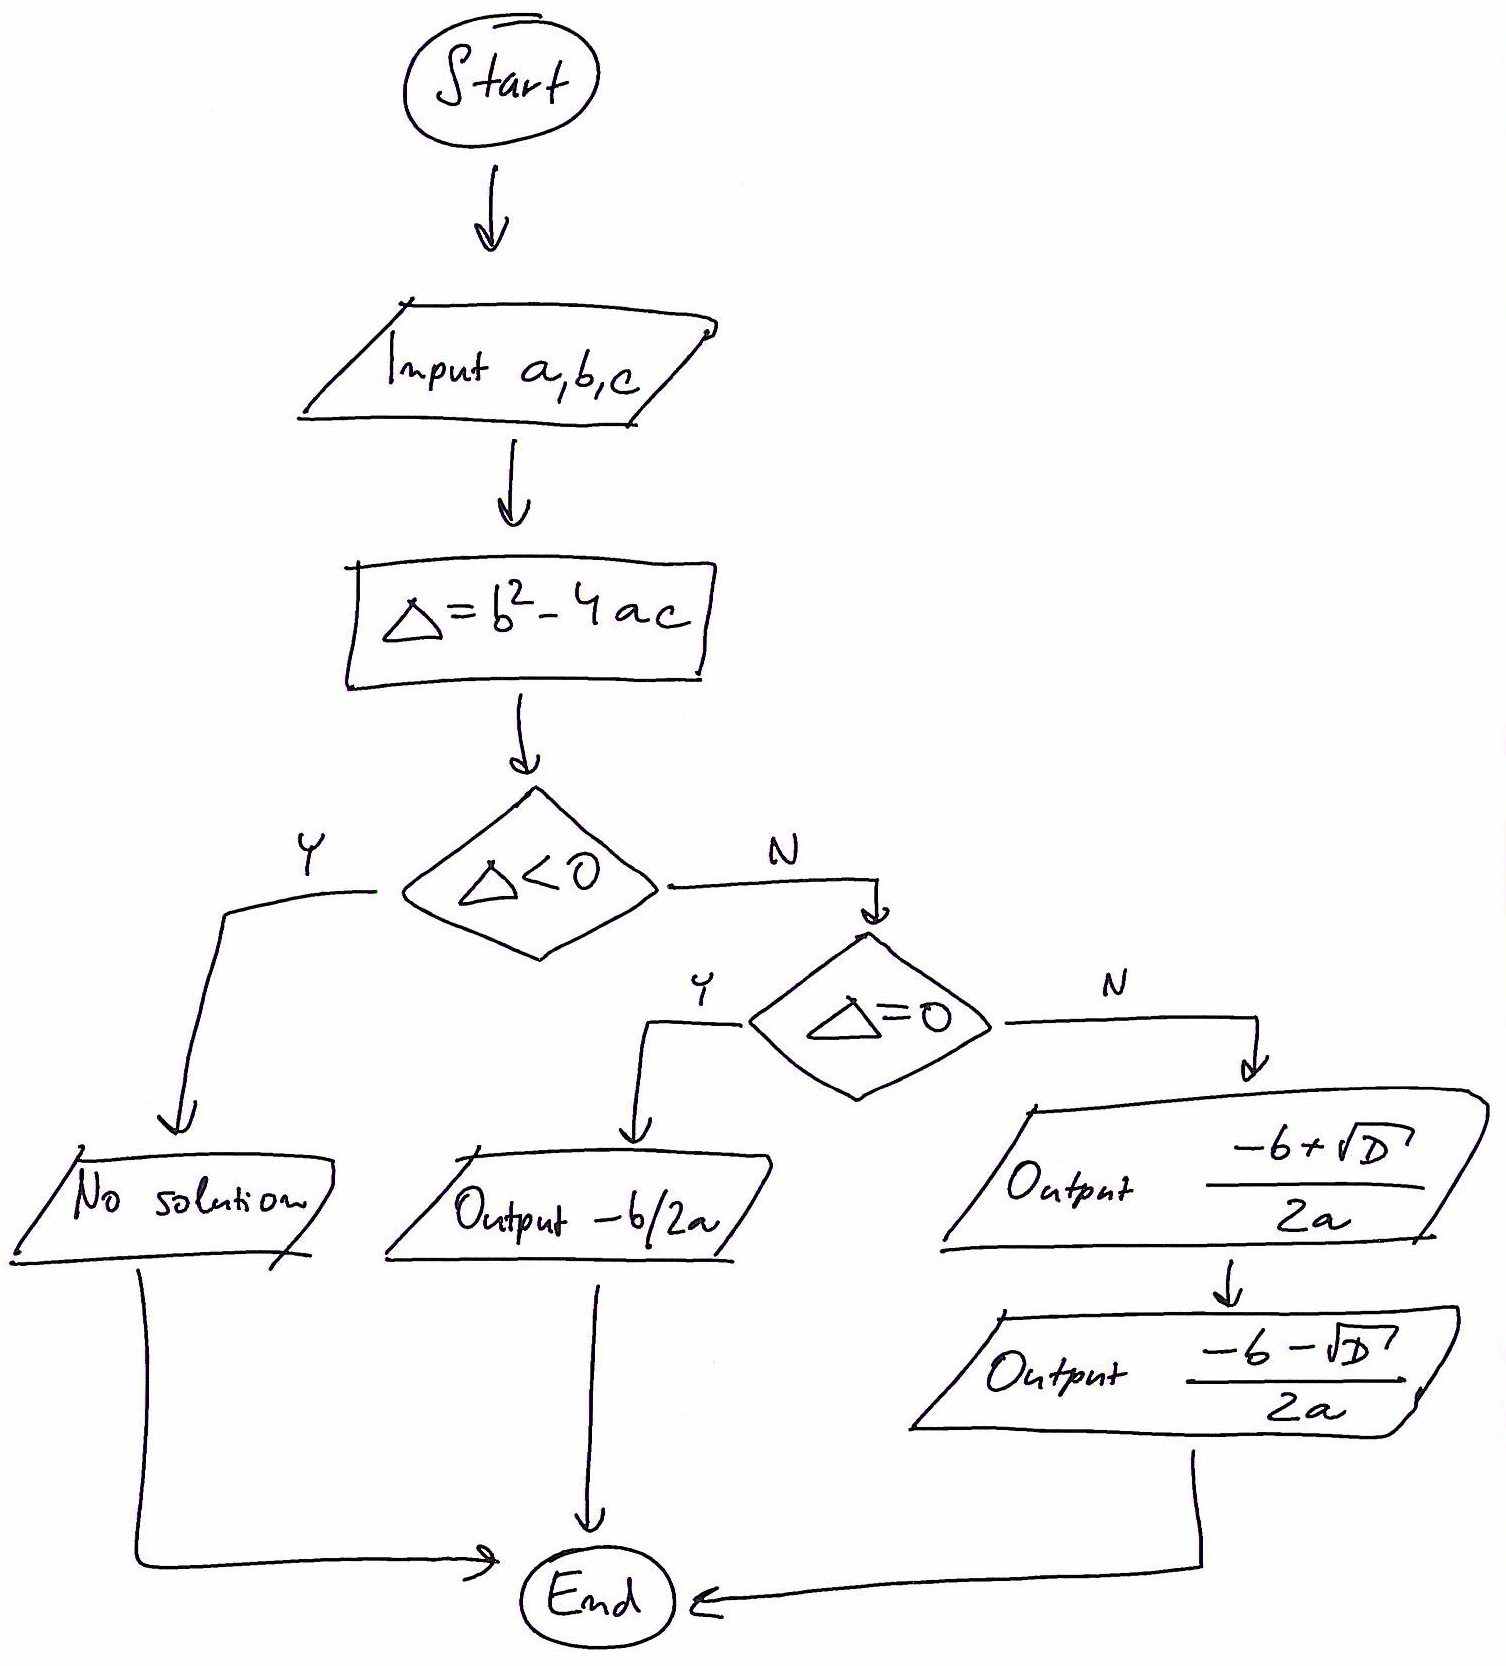
\includegraphics[width=0.44\linewidth]{ex5.png}}
    \hfill
    \subfloat[Structured output]{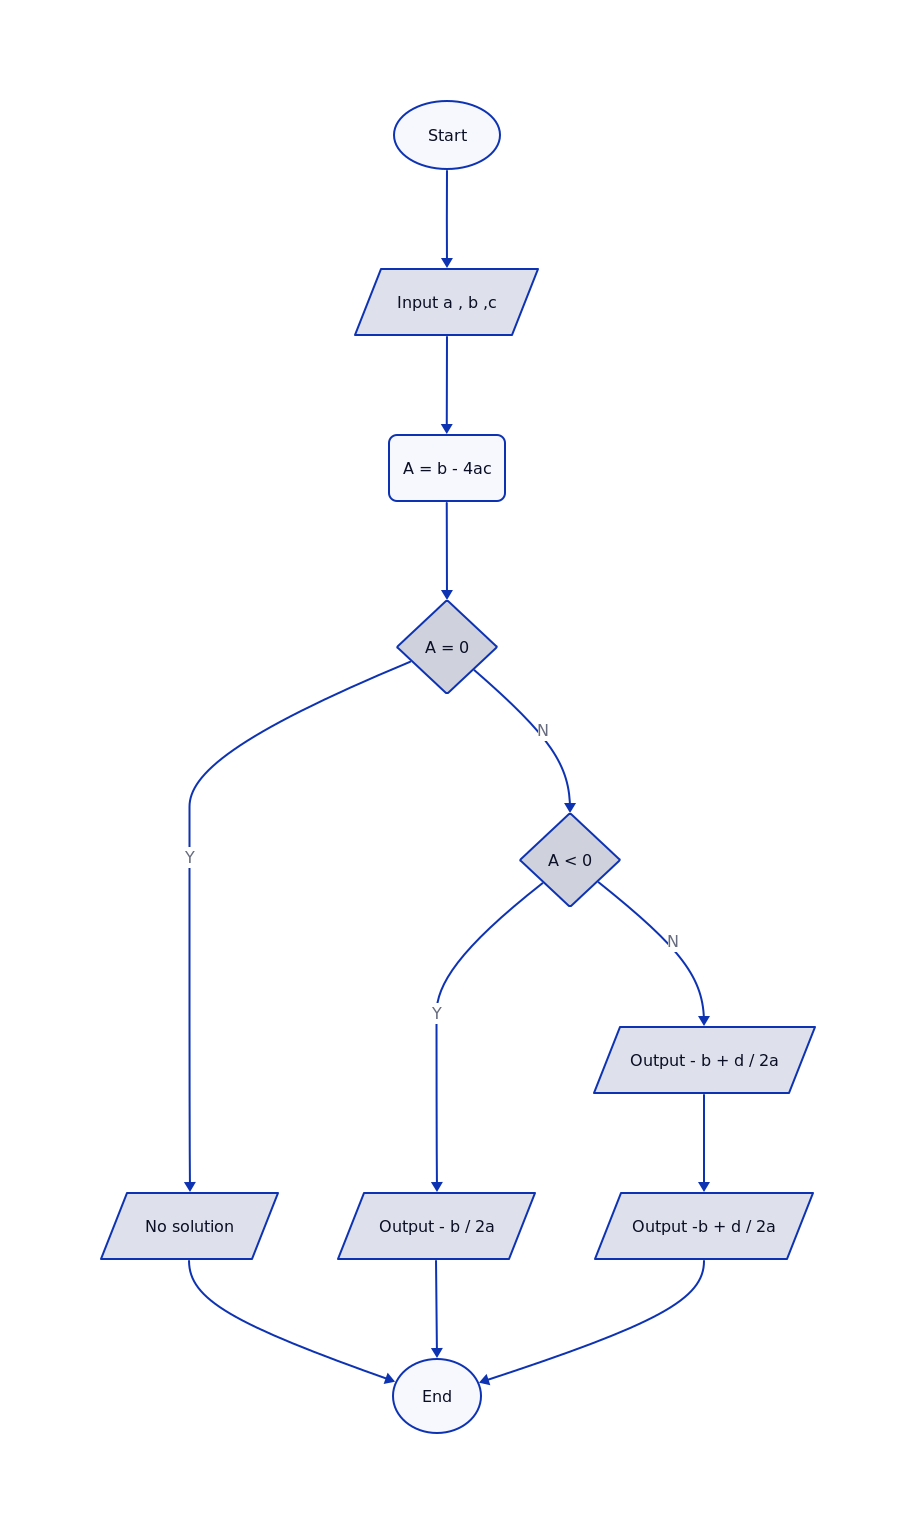
\includegraphics[width=0.24\linewidth]{ex6.png}}
    \caption{Representative end-to-end examples produced by DRAFT.}
    \label{fig:results}
\end{figure}

\begin{figure}[htbp]
    \centering
    \resizebox{\linewidth}{!}{%
    \begin{tabular}{ccc}
        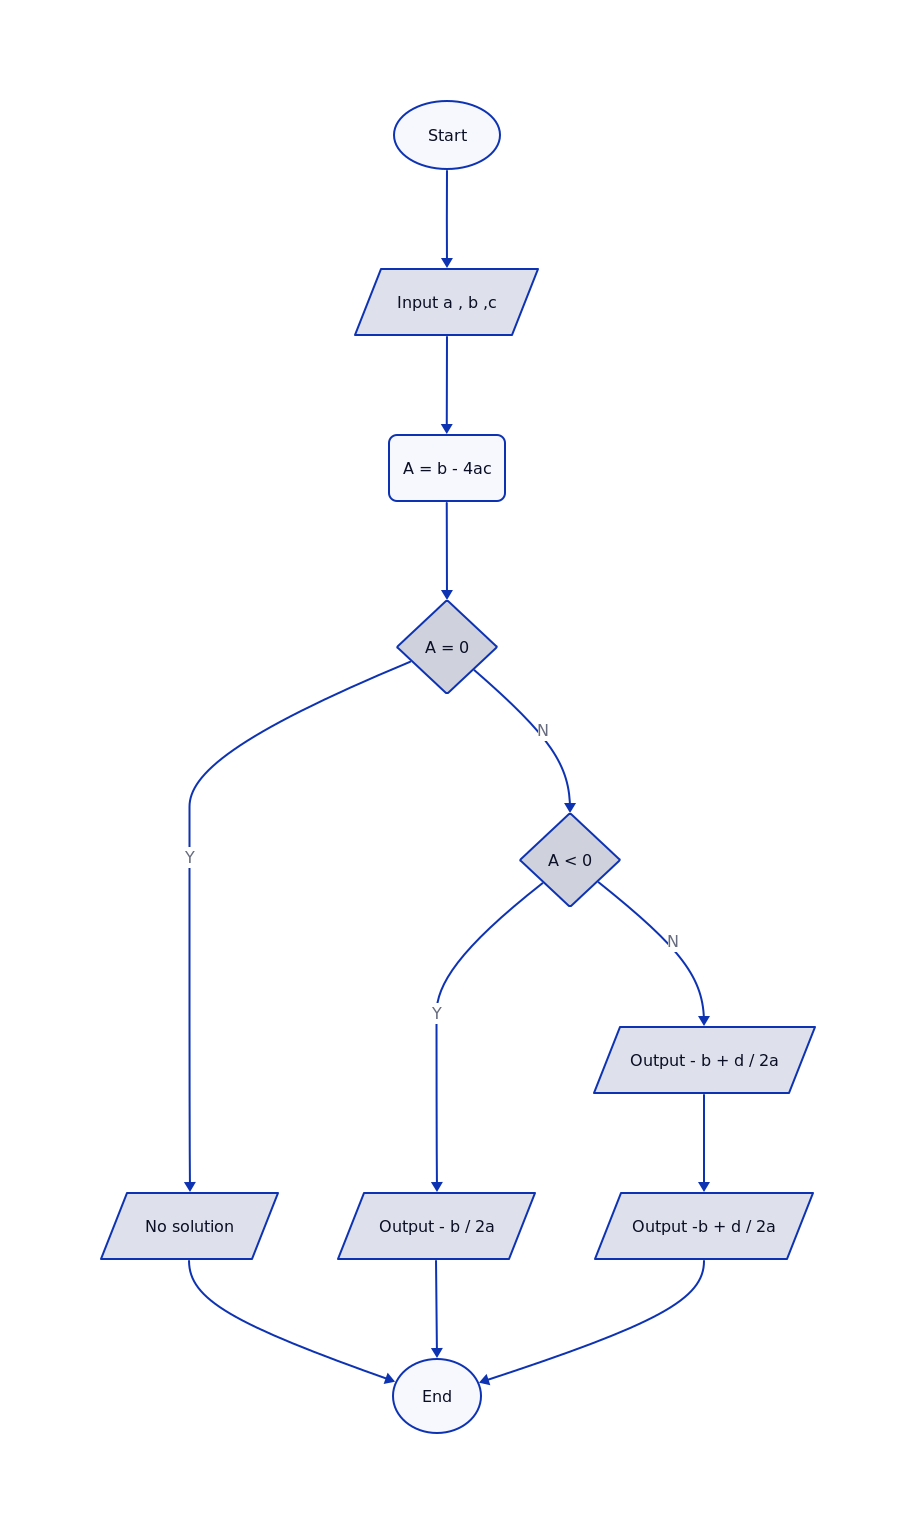
\includegraphics[height=4.8cm]{ex6.png} &
        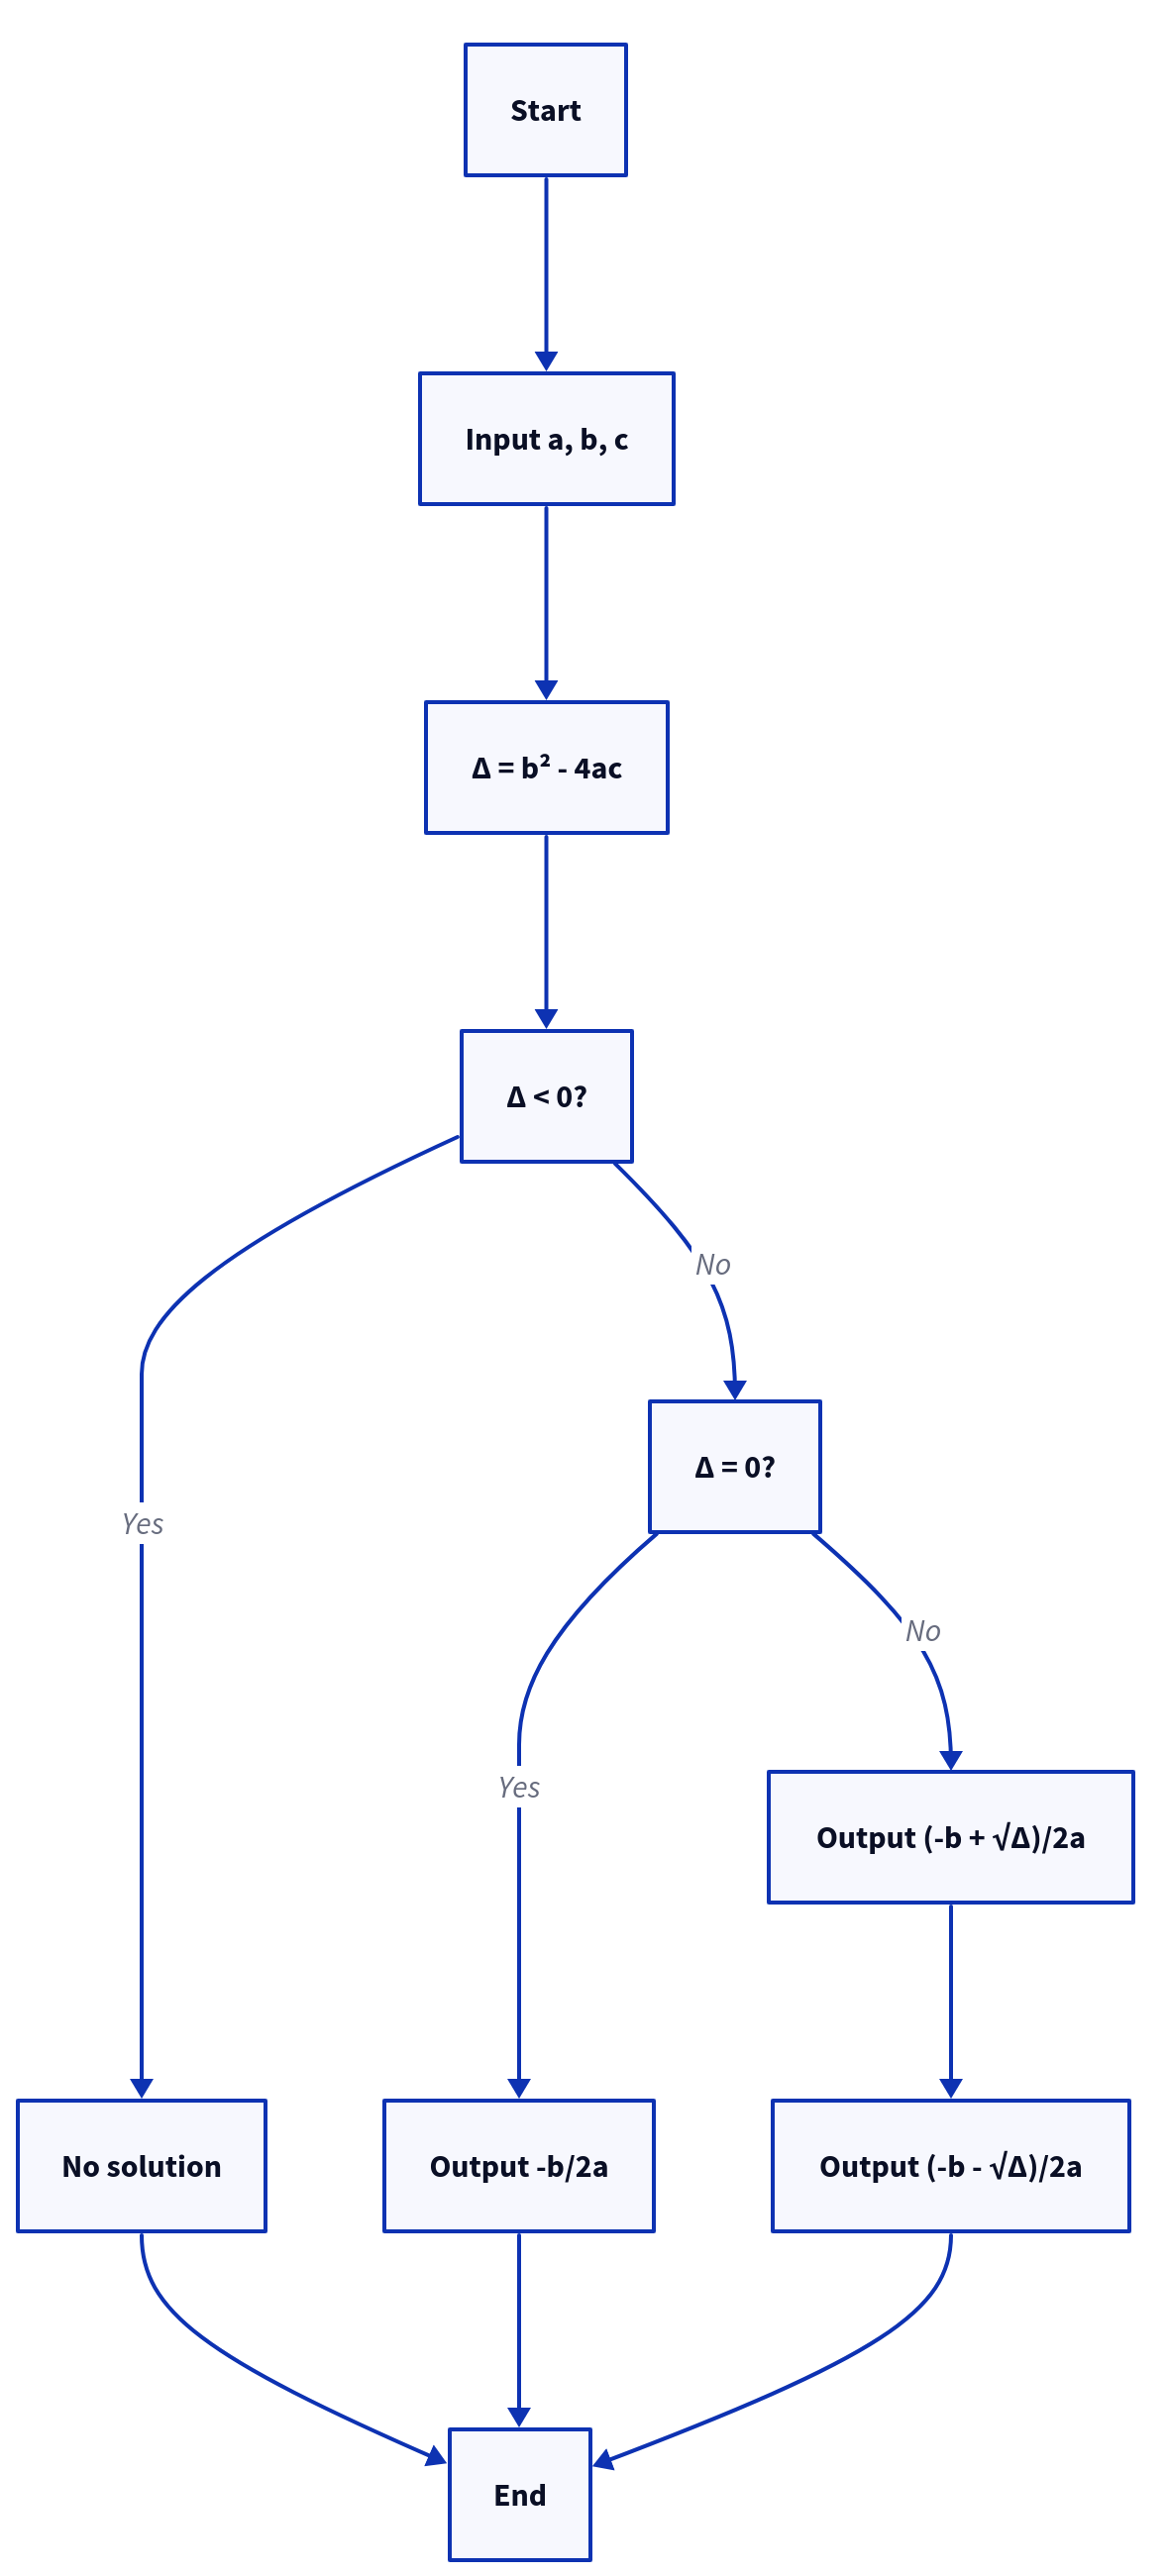
\includegraphics[height=4.8cm]{chat1.png} &
        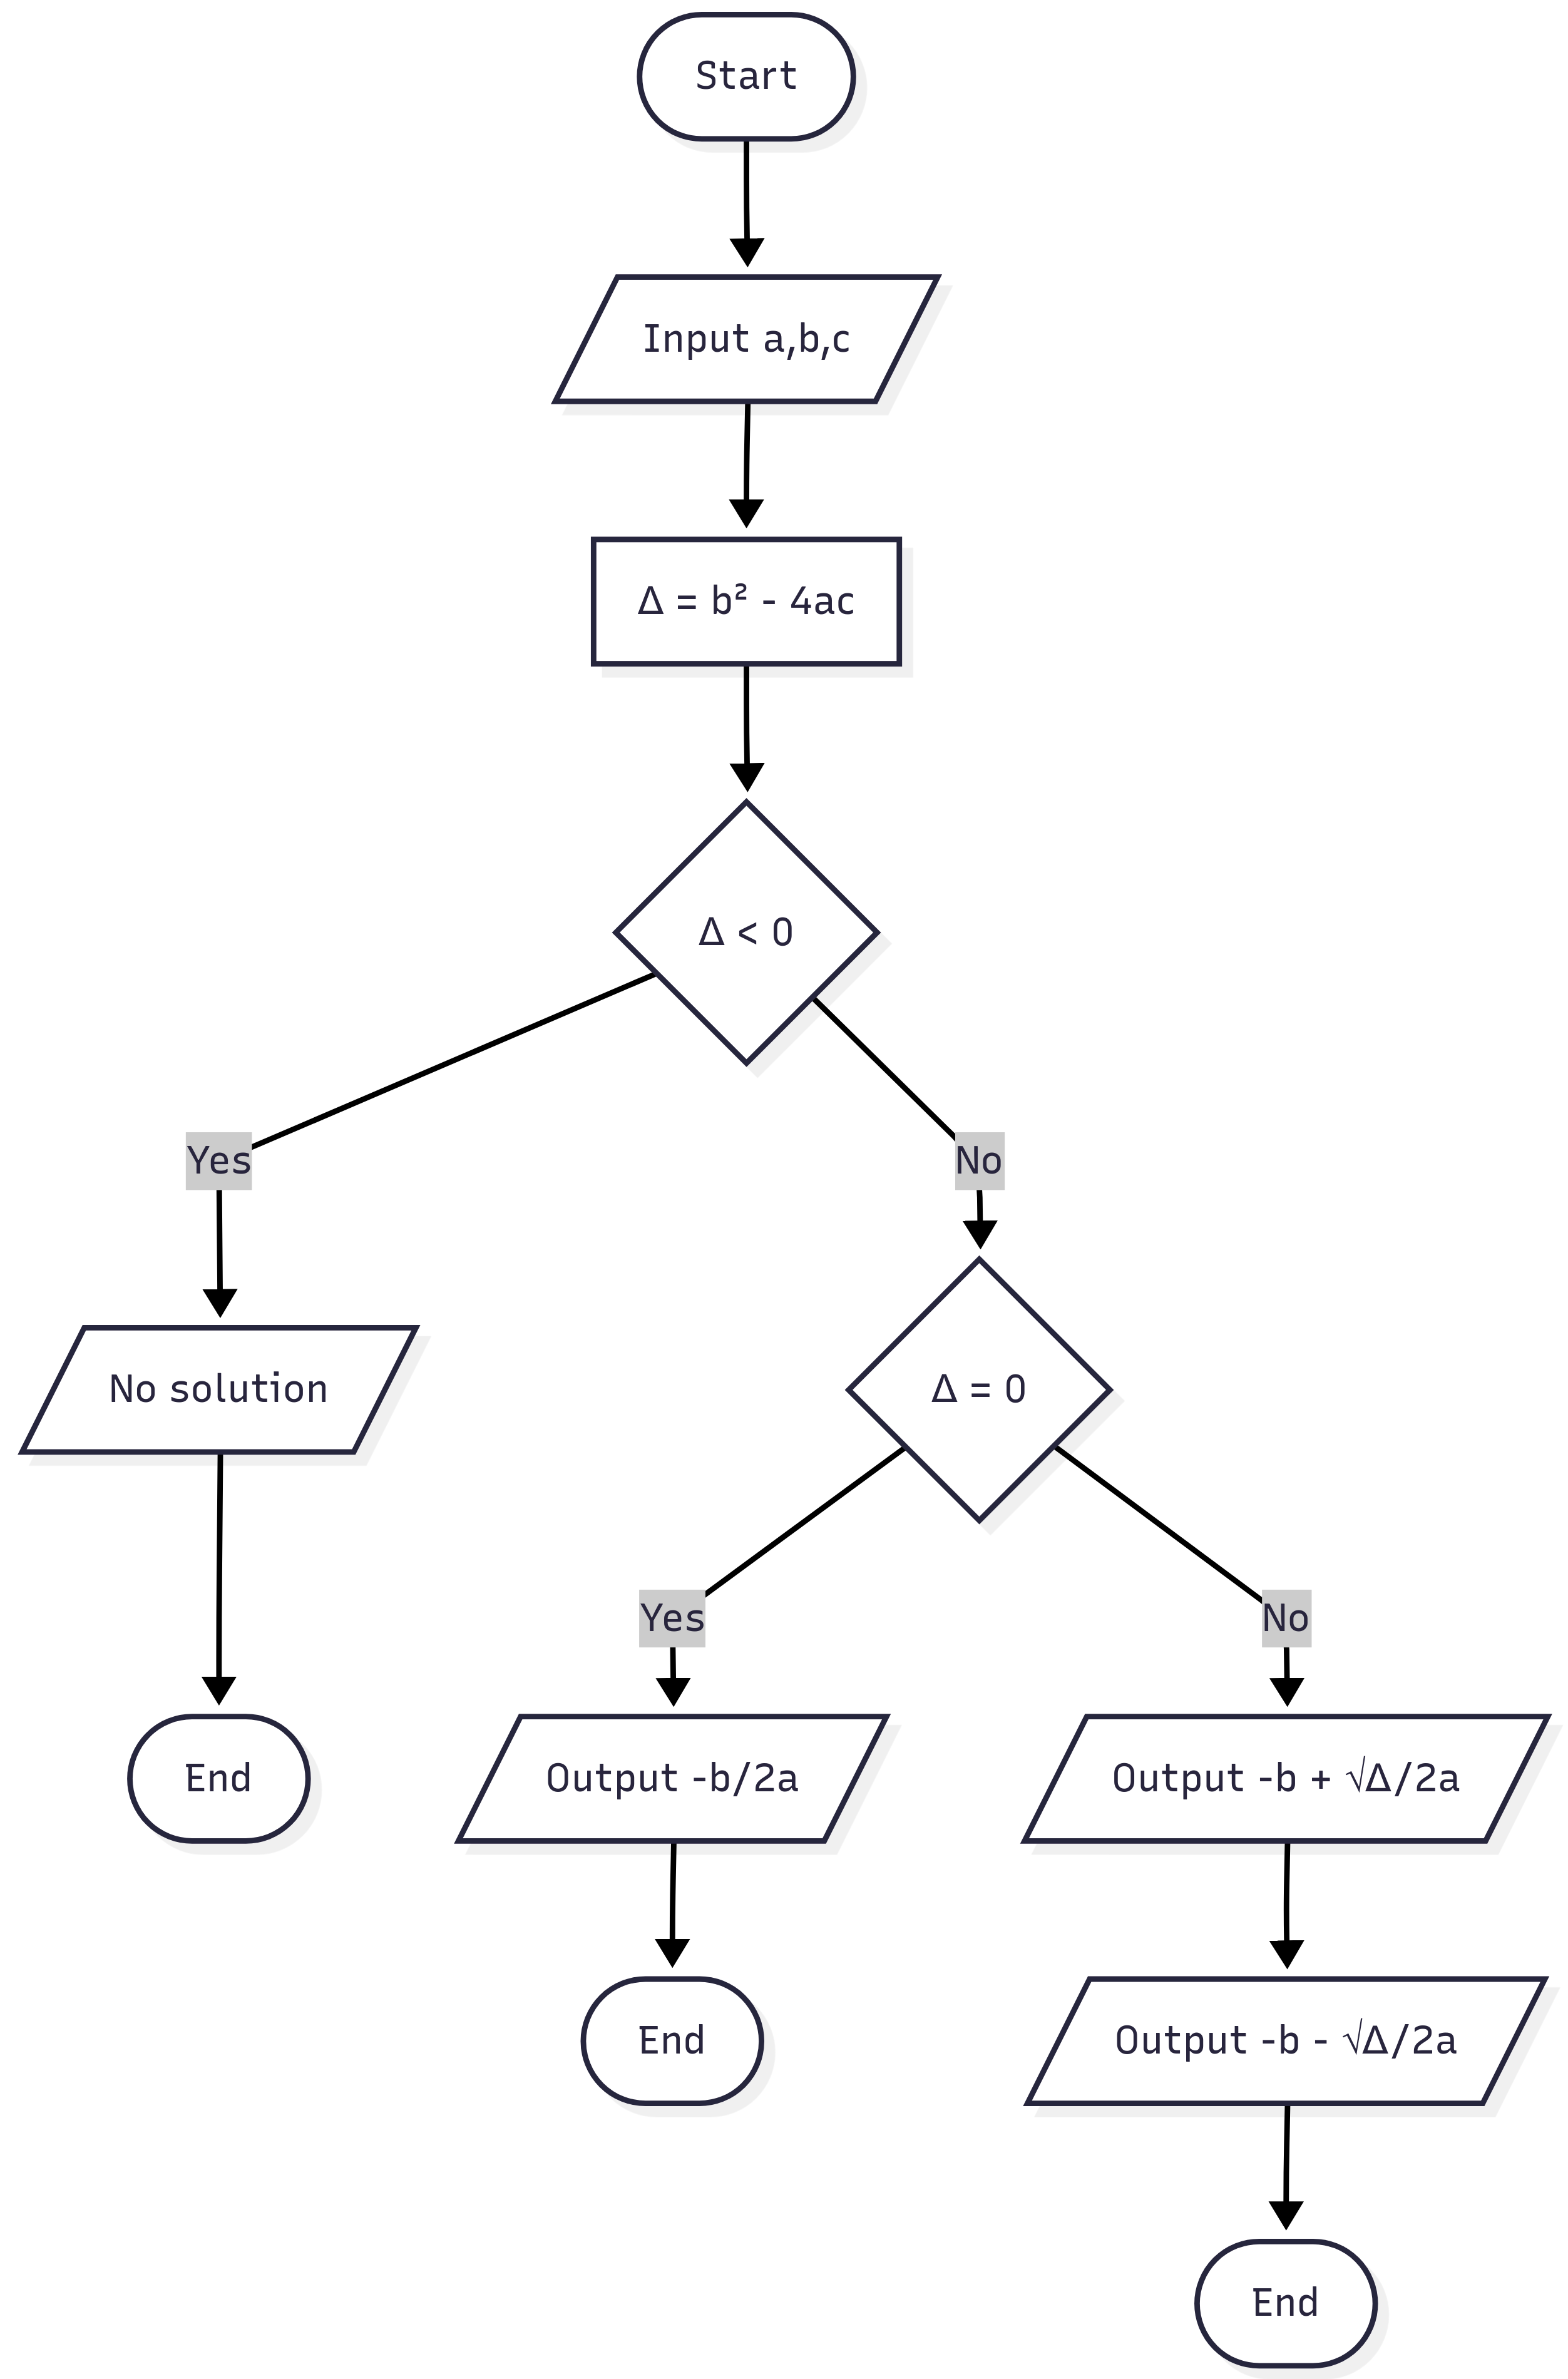
\includegraphics[height=4.15cm]{chat2.png} \\
        (a) Our result & (b) GPT Mermaid & (c) GPT D2 \\
    \end{tabular}}

    \vspace{0.6em}

    \resizebox{\linewidth}{!}{%
    \begin{tabular}{ccc}
        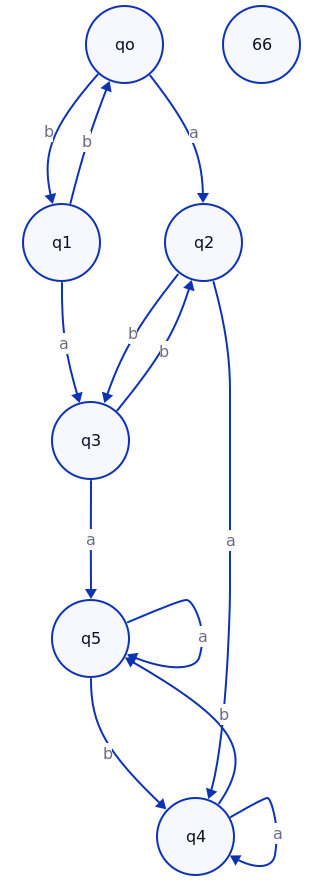
\includegraphics[height=4.8cm]{ex4.png} &
        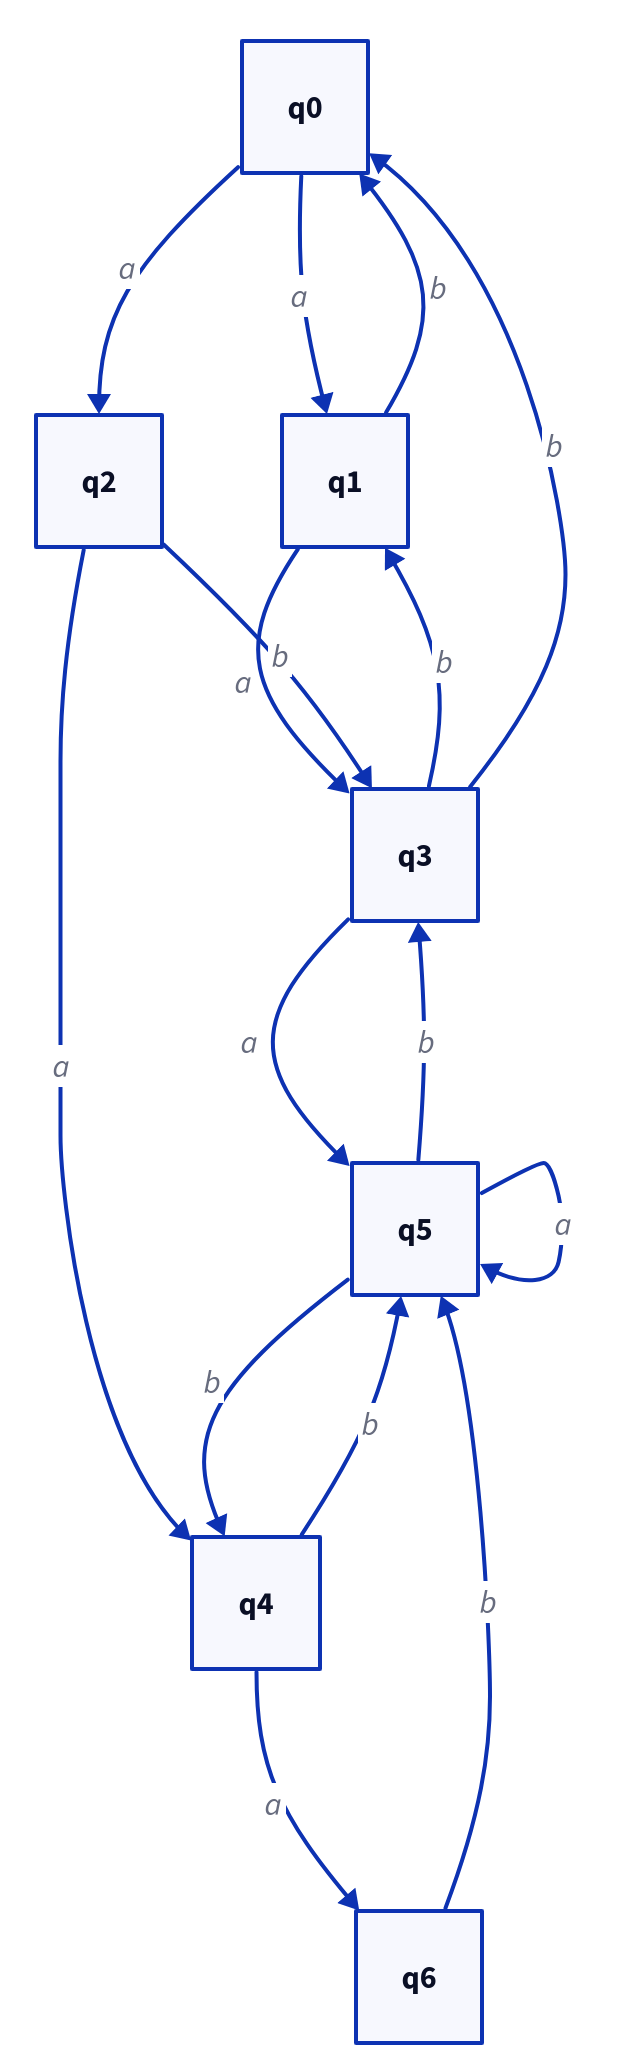
\includegraphics[height=4.8cm]{chat3.png} &
        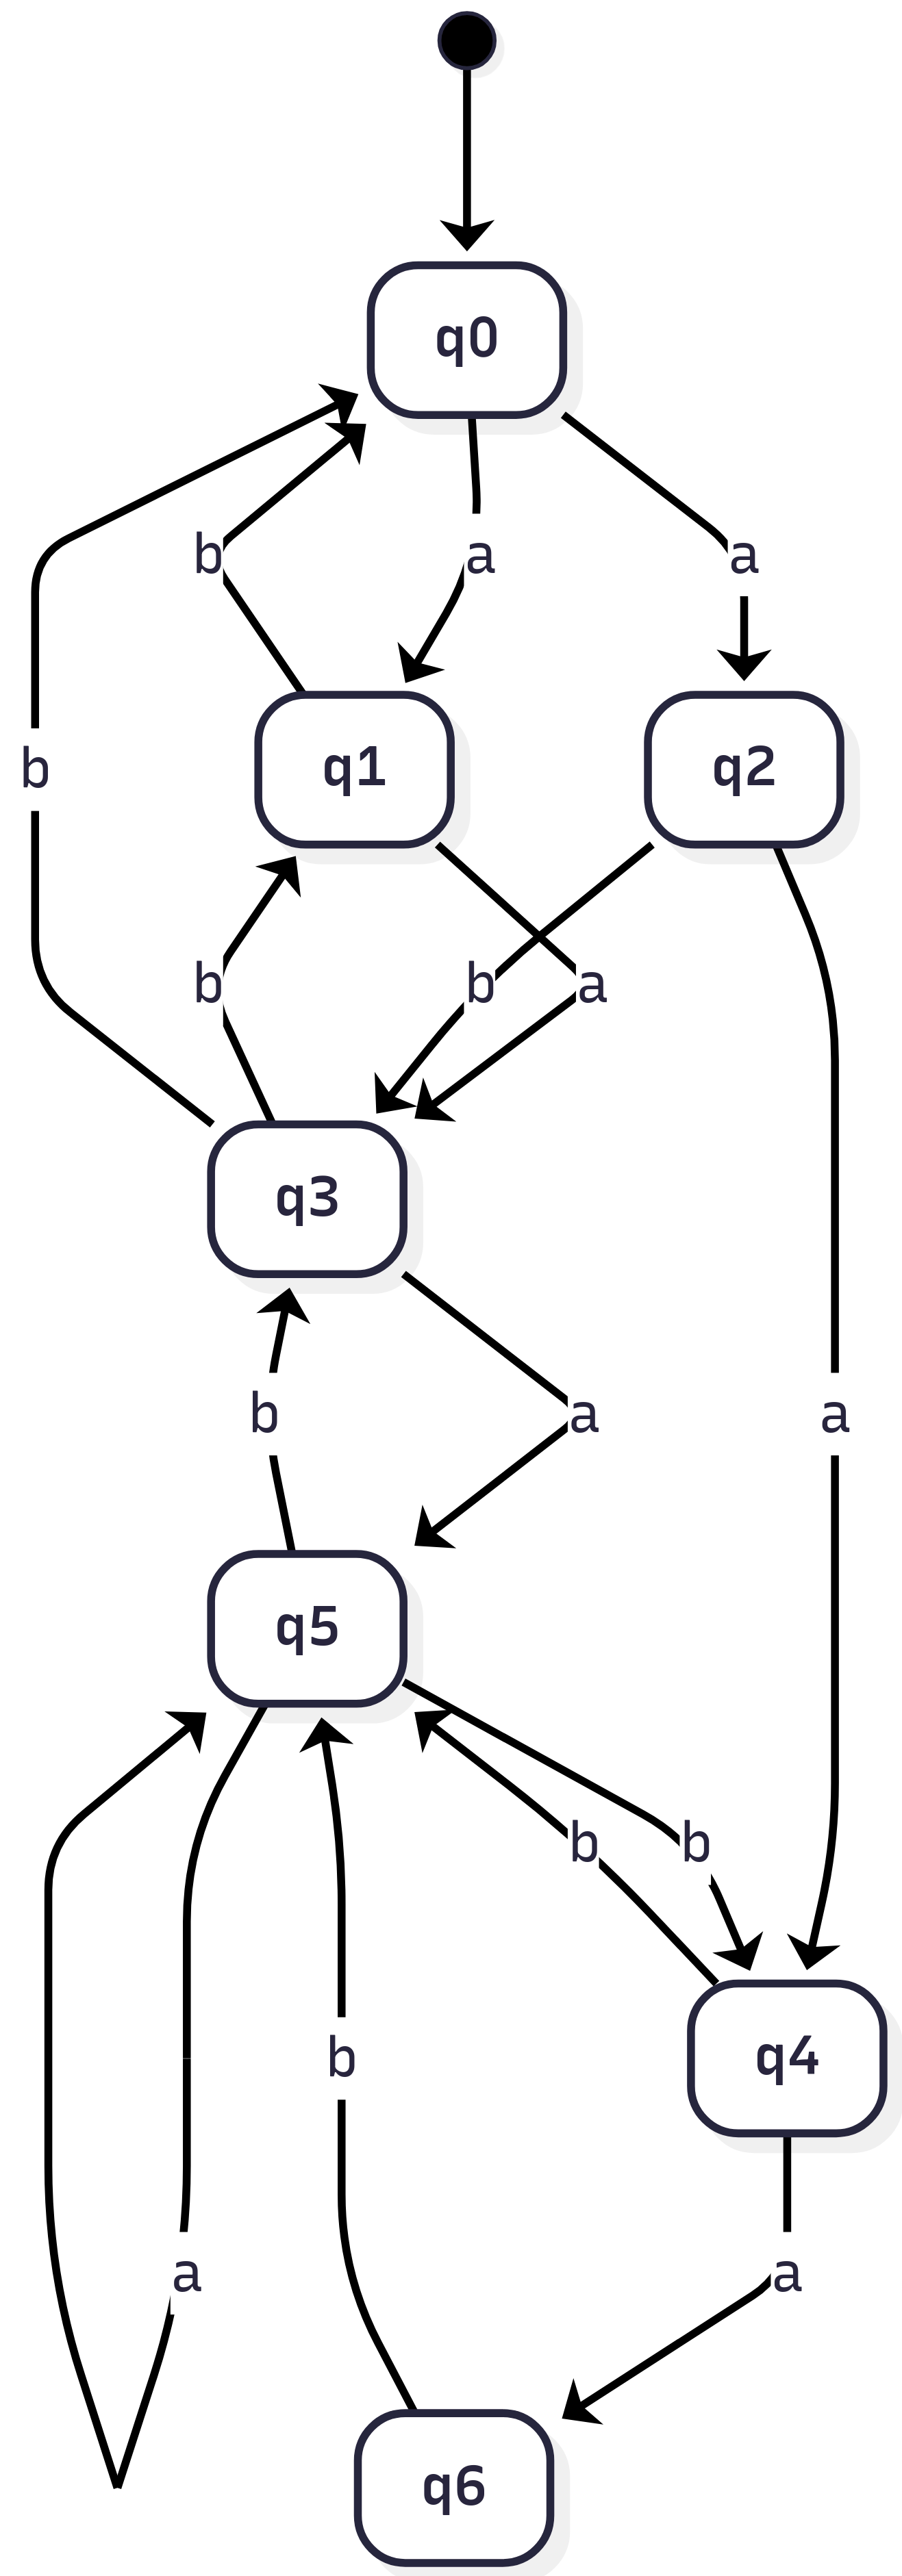
\includegraphics[height=4.8cm]{chat4.png} \\
        (d) Our result & (e) GPT Mermaid & (f) GPT D2 \\
    \end{tabular}}
    \caption{Qualitative comparison between DRAFT and zero-shot GPT-4o markup generation.}
    \label{fig:gpt_compare}
\end{figure}

\begin{figure}[htbp]
    \centering
    \subfloat[Zero-shot detector]{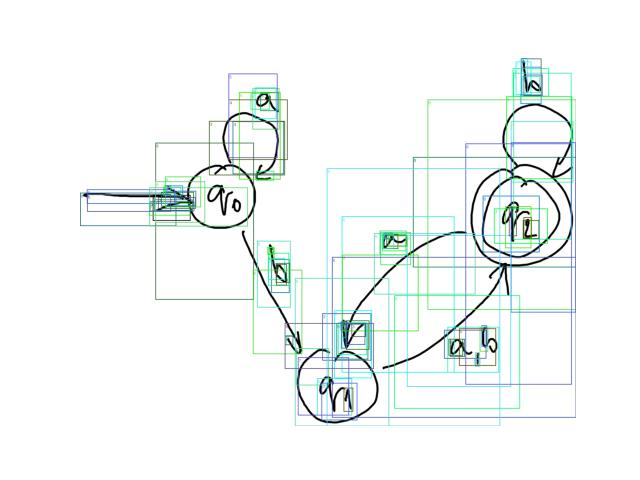
\includegraphics[width=0.31\linewidth]{bbox1.jpg}}
    \hfill
    \subfloat[Fine-tuned detector]{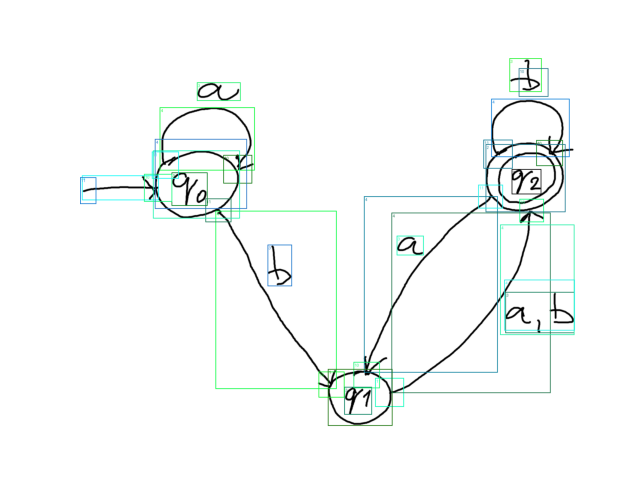
\includegraphics[width=0.28\linewidth]{bbox3.png}}
    \hfill
    \subfloat[Flowchart detection]{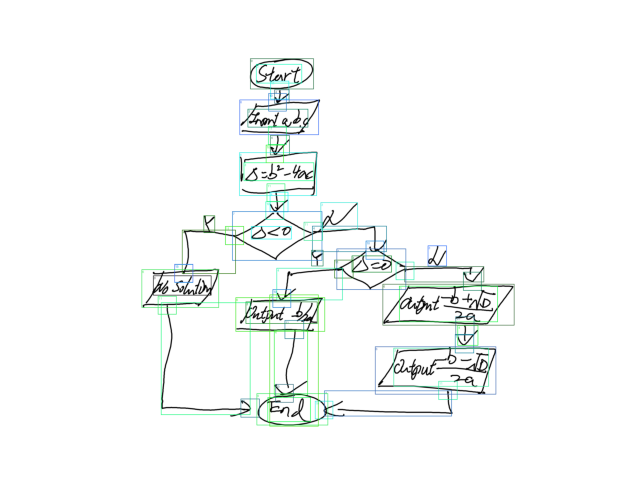
\includegraphics[width=0.28\linewidth]{fc.png}}
    \caption{Illustrative object-detection results before and after fine-tuning.}
    \label{fig:detection}
\end{figure}

Figure~\ref{fig:results} shows representative end-to-end examples for graph and flowchart inputs. Fig.~\ref{fig:gpt_compare} shows a qualitative comparison with zero-shot GPT-4o, prompted with: \textit{``The current image features a diagram. Analyze it and output the respective D2 and Mermaid script.''}. Three structural differences stand out. First, GPT-4o does not correctly preserve node shapes, whereas DRAFT\ explicitly detects and encodes element categories. Second, GPT-4o fails to correctly recognize self-arrows. Third, in one case GPT-4o generated three separate nodes from what was a single node in the original diagram. These differences matter in the educational setting because editable correctness — not visual similarity — is the goal. DRAFT is not without errors either: output~(d) in Fig.~\ref{fig:results} contains a spurious node in the upper-right corner, produced by the self-arrow NMS failure already described, illustrating that task-specific fine-tuning reduces but does not eliminate structural errors.

Figure~\ref{fig:detection} highlights the role of task-specific fine-tuning in the extractor. The zero-shot detector identifies only part of the structure, whereas the fine-tuned model recovers more complete node and arrow information. This behavior is important in the educational setting because downstream usability depends on preserving the logical structure of the original sketch.

\section{Discussion}
The main result of this work is the successful design of a complete pipeline that transforms handwritten diagrams into structured, editable representations. The extractor was the strongest component, validating fine-tuned deep networks for this subtask; the classifier was more sensitive to class imbalance, and the modular design allows new diagram categories to be added without redesigning the pipeline. Compared to online recognition methods, the system addresses the harder offline setting — image-only, no stroke trajectory — while producing structured output, positioning it as a hybrid between rule-based and learned components.

The present work does not include a classroom study or a quantitative evaluation of learning outcomes. Therefore, the contribution addresses technical feasibility rather than pedagogical effectiveness. Technically, the system remains constrained by dataset size, class imbalance, and handwritten input variability; more broadly, all pipeline stages assume a degree of input neatness that may not be guaranteed in uncontrolled real-world capture conditions. Observed failure modes include: (1) self-arrows in graph diagrams, where the curved ink is occasionally classified as a node with higher confidence than as an arrow — NMS does not resolve this since the node class wins the confidence comparison and the spurious detection survives — with low self-arrow representation in training data as the root cause; (2) small-object detection, which degrades at mAP 0.6444 for fine-grained diagram elements; and (3) text association failures on densely annotated diagrams, where distance-based heuristics are less reliable.

\section{Integration Opportunities}
DRAFT is relevant for programming, automata, control, and software engineering courses where students sketch diagrams during exercises. A practical revision workflow has students submit a photographed sketch, inspect or correct the Mermaid or D2 output, and turn in the structured result — reducing transcription effort while encouraging reflection on formal diagram structure. A secondary use case is instructor-side archiving; a longer-term direction is semi-automatic formative feedback, for which the system provides the necessary prerequisite: a machine-readable representation of handwritten student work.

\section{Arrow Orientation: Design Iterations}
Determining the head and tail of a detected arrow proved to be a non-trivial design challenge. Two approaches were explored and discarded before reaching the final design.

The first approach, \textit{Double Clustering}, operated entirely within each arrow bounding box: SIFT keypoints were extracted, DBSCAN or Spectral Clustering was applied to isolate the arrow stroke from background noise (Fig.~\ref{fig:dc_process}a), the two most distant keypoints within the main cluster were taken to estimate arrow direction (Fig.~\ref{fig:dc_process}b), and template matching was run near each endpoint to identify the head. This approach failed systematically on self-arrows, where the curved ink caused the maximum-distance heuristic to yield endpoints unrelated to the actual head and tail (Fig.~\ref{fig:dc_process}b); template matching also proved sensitive to handwriting style variation across the dataset.

\begin{figure}[htbp]
    \centering
    \subfloat[Direction from max-distance keypoints]{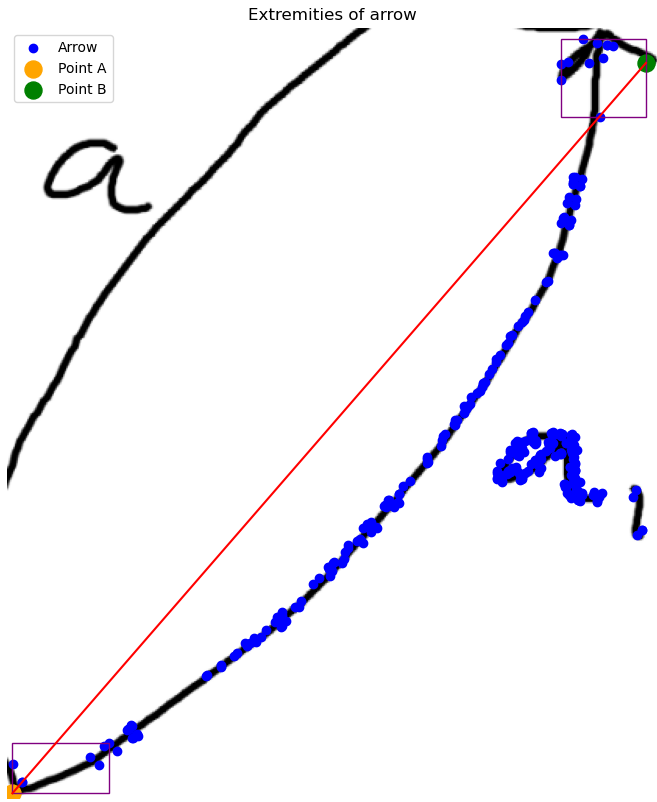
\includegraphics[width=0.45\linewidth]{arrow_double_clustering_direction.png}}
    \hfill
    \subfloat[Self-arrow: extremities miss actual head/tail]{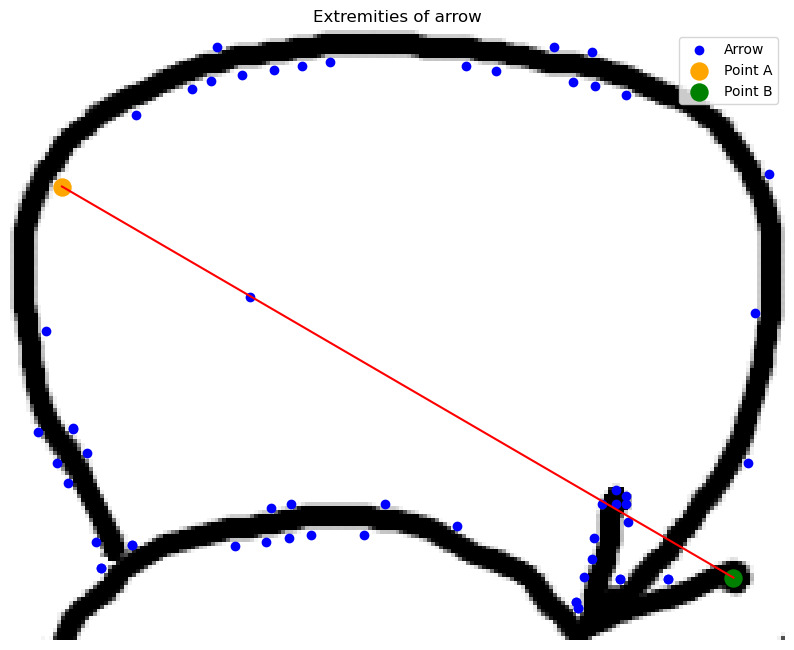
\includegraphics[width=0.45\linewidth]{selfarrowdc.jpg}}
    \caption{Double Clustering: (a) direction estimate (red line) between most distant SIFT keypoints in main cluster; (b) failure on self-arrow — arc geometry displaces detected extremities from actual head/tail.}
    \label{fig:dc_process}
\end{figure}

The second approach, \textit{ArrowNet}, used a lightweight UNet-inspired encoder-decoder to directly segment the arrow bounding box and predict head and tail point heatmaps. Two output channels — one for head presence, one for tail presence — were trained using synthetic annotations. Training on the available synthetic samples caused the network to overfit to ink density rather than learning orientation-sensitive features, producing predictions that simply highlighted regions of dark ink regardless of arrow direction. The architecture comprised a two-stage encoder (32 and 64 channels), a 128-channel bottleneck, a symmetric decoder, and a two-channel $1{\times}1$ output convolution — one channel per endpoint. The root failure was a domain gap: rendered synthetic arrows cannot substitute for real annotated handwritten samples.

The final solution — extending the Faster R-CNN fine-tuning to also detect separate bounding boxes for arrow heads and arrow tails — was both simpler and more robust. It leveraged the same detection framework already used for node and arrow-body localization, required no additional architecture, and produced orientation labels that compose naturally with the rest of the relation-building pipeline.

\section{Classroom Deployment Considerations}
The current CLI-based workflow is intentionally human-in-the-loop: a student submits a photographed sketch, receives a first-pass Mermaid or D2 rendering, and corrects errors before submission — a better fit for early adoption than a black-box autograder, since detection or OCR mistakes can be fixed directly in the editable output. Pretrained weights are publicly released for local trials without retraining. Future steps include a web interface and comparison of generated diagrams against reference structures for formative feedback.

\section{Conclusion}
DRAFT demonstrates the feasibility of converting handwritten engineering diagrams into structured and editable digital representations through a hybrid pipeline combining learned and deterministic components. DRAFT supports a complete workflow from image input to Mermaid or D2 output. Source code and pretrained model weights are publicly available at \url{https://github.com/diagram-framework/draft}, with weights hosted at a linked public folder to allow end-to-end reproduction without retraining from scratch.

This work demonstrates technical feasibility; pedagogical effectiveness requires dedicated classroom study. The most realistic near-term role of DRAFT is assisted digitization under human supervision — allowing students or instructors to inspect and correct generated structures before reuse, submission, or feedback. Future studies should evaluate recognition quality, revision effort, and the usefulness of structured outputs for formative feedback; technical improvements include data augmentation to address classifier fragility, parallelization of the extractor pipeline, and Docker containerization.

\bibliographystyle{IEEEtran}
\bibliography{../../article/article}

\end{document}
